\documentclass[12pt, a4paper]{article}

% ── Pacotes ─────────────────────────────────────────────────
\usepackage[utf8]{inputenc}
\usepackage[T1]{fontenc}
\usepackage[brazil]{babel}
\usepackage{geometry}
\usepackage{setspace}
\usepackage{indentfirst}
\usepackage{titlesec}
\usepackage{titling}
\usepackage{booktabs}
\usepackage{array}
\usepackage{longtable}
\usepackage{hyperref}
\usepackage{graphicx}
\usepackage{fancyhdr}
\usepackage{enumitem}
\usepackage{xcolor}
\usepackage{parskip}

% ── Geometria da página ──────────────────────────────────────
\geometry{
  top    = 3cm,
  bottom = 2cm,
  left   = 3cm,
  right  = 2cm
}

% ── Espaçamento ──────────────────────────────────────────────
\onehalfspacing
\setlength{\parindent}{1.25cm}

% ── Formatação de seções ─────────────────────────────────────
\titleformat{\section}[block]
  {\normalfont\large\bfseries\MakeUppercase} 
  {\thesection.}{0.5em}{}
  
\titleformat{\subsection}[block]
  {\normalfont\normalsize\bfseries}
  {\thesubsection.}{0.5em}{}

\titlespacing*{\section}{0pt}{1.5ex plus .2ex}{1ex plus .2ex}
\titlespacing*{\subsection}{0pt}{1ex plus .2ex}{0.5ex plus .2ex}

% ── Hiperlinks ───────────────────────────────────────────────
\hypersetup{
  colorlinks = true,
  linkcolor  = black,
  urlcolor   = blue,
  citecolor  = black
}

% ── Cabeçalho / rodapé ───────────────────────────────────────
\pagestyle{fancy}
\fancyhf{}
\rhead{\small Gestão da Produção e Qualidade}
\lhead{\small GPeQ – Grupo 03}
\rfoot{\thepage}
\renewcommand{\headrulewidth}{0.4pt}

% ============================================================
\begin{document}

% ── CAPA ────────────────────────────────────────────────────
\begin{titlepage}
  \centering

  {\large \textbf{UNIVERSIDADE DE BRASÍLIA}}\\[0.3cm]
  {\large Faculdade do Gama – FGA}\\[2cm]

  {\Large \textbf{GESTÃO DA PRODUÇÃO E QUALIDADE}}\\[0.5cm]
  {\large Professora: Rejane Figueiredo}\\[2cm]

  {\Large \textit{Relatório de Visita Técnica: Avaliação Operacional e Análise da Produção do Prato de Parmegiana de Carne no Restaurante e Bar Tarumã}}\\[2cm]

  {\large \textbf{Grupo 03}}\\[1cm]

\end{titlepage}
 
% ── FOLHA DE ROSTO ──────────────────────────────────────────
\begin{titlepage}
  \centering

  \begin{tabular}{cc}
    
\includegraphics[width=0.22\textwidth]{imagens/integrantes/Tiago_Geovane_da_Silva_Sousa.png} & 
\includegraphics[width=0.22\textwidth]{imagens/integrantes/Henrique_Mendes_Elias.png} \\
    Integrante 1 - Tiago Geovane & Integrante 2 - Henrique Mendes \\[0.5cm]
    
\includegraphics[width=0.22\textwidth]{imagens/integrantes/João_Guilherme_Amancio_de_Melo.png} & 
\includegraphics[width=0.22\textwidth]{imagens/integrantes/Gabriel_Portácio_Candeia_Costa.png} \\
    Integrante 3 - João Guilherme & Integrante 4 - Gabriel Portácio \\[0.5cm]
    
\includegraphics[width=0.22\textwidth]{imagens/integrantes/Guilherme_Gusmão_Nepomuceno.png} & 
\includegraphics[width=0.22\textwidth]{imagens/integrantes/Matheus_Rodrigues_Pontes.png} \\
    Integrante 5 - Guilherme Gusmão & Integrante 6 - Matheus Rodrigues \\
  \end{tabular}\\[1.5cm]

  \hfill
  \begin{minipage}{0.5\textwidth}
    Relatório de visita técnica apresentado como requisito parcial de avaliação da disciplina de Gestão da Produção e Qualidade, do curso de engenharia da Faculdade do Gama (FGA), da Universidade de Brasília (UnB).
    
    \vspace{0.5cm}
    \textbf{Professora:} Rejane Figueiredo
  \end{minipage}

  \vfill

  {\large Brasília, \today}

\end{titlepage}

% ── Sumário ──────────────────────────────────────────────────
\tableofcontents
\newpage

% ============================================================
% 1. INTRODUÇÃO
% ============================================================
\section{Introdução}

A Administração da Produção e Operações pode ser definida, baseando-se nos conceitos de Krajewski \textit{et al.}, como o projeto, a direção e o controle sistemáticos dos processos que transformam insumos em serviços e produtos para clientes internos e externos. Compreender e otimizar tais processos é um aspecto fundamental para assegurar a eficiência, a qualidade e a competitividade de qualquer organização, o que se aplica diretamente ao setor de serviços de alimentação.

Neste contexto, o presente documento tem como principal objetivo apresentar e estruturar os dados coletados durante uma visita técnica realizada no Restaurante e Bar Tarumã, atividade proposta pela disciplina de Gestão da Produção e Qualidade. O estudo teve como foco a observação e análise detalhada do processo de produção de um de seus pratos: a parmegiana de carne.

Por meio da coleta de dados in loco, buscou-se não apenas documentar as etapas práticas do preparo — identificando as especificações de entrada como recursos transformadores e transformados —, mas também analisar a operação sob a ótica gerencial. Dessa forma, o relatório visa relacionar a realidade prática do restaurante com os fundamentos teóricos abordados na disciplina, como a estratégia da produção e o escopo das operações, proporcionando uma compreensão abrangente de como a gestão de processos impacta diretamente na entrega final ao cliente.

% ============================================================
% 2. ESPECIFICAÇÕES DE ENTRADA
% ============================================================
\section{Especificações de Entrada}

\subsection{Recursos Transformadores}

\subsubsection*{Funcionários}

No processo de produção e entrega do prato, desde a captação do pedido até o serviço na mesa, os recursos humanos atuam diretamente na prestação do serviço e na manipulação das matérias-primas. Os principais funcionários envolvidos são:

\begin{itemize}
    \item \textbf{Garçom / Atendente:} Responsável pela interface direta com o cliente. Ele capta o pedido, esclarece dúvidas sobre o prato, insere os dados no sistema para envio à cozinha e, ao final do processo, entrega o prato finalizado na mesa.
    \item \textbf{Auxiliar de Cozinha:} Encarregado do pré-preparo (\textit{mise en place}). Realiza atividades como higienizar, descascar e cortar as batatas, separar as porções de carne, preparar as estações de empanamento e auxiliar na limpeza do ambiente.
    \item \textbf{Cozinheiro:} Profissional responsável pela transformação térmica e química dos ingredientes. Ele tempera e empana o bife, realiza a fritura da carne e das batatas, cozinha o arroz, prepara o molho de tomate e faz a montagem das camadas (carne, molho, queijo).
    \item \textbf{Expedidor ou Chefe de Cozinha (dependendo do porte do restaurante):} Responsável por fazer o controle de qualidade visual e de temperatura antes de liberar o prato pronto da cozinha para o garçom.
\end{itemize}

\subsubsection*{Máquinas e Equipamentos}

As instalações, máquinas e equipamentos formam a infraestrutura tecnológica e física necessária para que os funcionários executem o trabalho. A lista inclui desde a área de tecnologia até o maquinário pesado da cozinha:

\begin{itemize}
    \item \textbf{Sistema de PDV (Ponto de Venda) e Impressora/Monitor de Pedidos:} Hardware e software utilizados pelo garçom para registrar o pedido e transmiti-lo instantaneamente para a cozinha, iniciando o fluxo de produção.
    \item \textbf{Refrigeradores e Freezers Industriais:} Equipamentos que mantêm a matéria-prima (carnes, queijos, presunto) em temperatura segura até o momento do uso.
    \item \textbf{Bancadas de Aço Inox e Tábuas de Corte:} Superfícies padronizadas para manipulação segura e higiênica dos alimentos durante o \textit{mise en place}.
    \item \textbf{Fritadeira Industrial (Elétrica ou a Gás):} Equipamento crítico do processo, utilizado para fritar os bifes empanados e as batatas por imersão, garantindo rapidez e crocância com temperatura controlada.
    \item \textbf{Fogão Industrial:} Utilizado para o cozimento do arroz e para a cocção e redução do molho de tomate.
    \item \textbf{Forno Industrial ou Salamandra:} Equipamento de finalização utilizado exclusivamente para derreter o queijo e gratinar o prato de forma rápida e uniforme antes de ser servido.
    \item \textbf{Utensílios de Cozinha Gerais:} Panelas, escumadeiras, facas, pinças e cubas gastronômicas essenciais para o manuseio dos alimentos ao longo de todas as etapas.
\end{itemize}

\subsection{Recursos Transformados}
No processo de preparação do prato de parmegiana de carne, que consiste em arroz cozido, batatas fritas e o bife de carne à parmegiana, os recursos transformados consistem nos ingredientes do prato, que são os seguintes:

\begin{itemize}
    \item \textbf{Para o bife à parmegiana:} 
    \begin{itemize}
        \item Bifes de carne bovina;
        \item Temperos (sal, pimenta-do-reino e alho);
        \item Ingredientes para empanar (farinha de trigo, ovos batidos e farinha de rosca);
        \item Óleo (para a fritura);
        \item Molho de tomate;
    \end{itemize}
    
    \item \textbf{Para o arroz:}
    \begin{itemize}
        \item Arroz branco (agulhinha);
        \item Óleo ou azeite;
        \item Alho e cebola picados;
        \item Sal;
        \item Água.
    \end{itemize}
    
    \item \textbf{Para as batatas fritas:}
    \begin{itemize}
        \item Batatas;
        \item Óleo (para a fritura);
        \item Sal.
    \end{itemize}
\end{itemize}


% ============================================================
% 3. ESTRATÉGIA DA PRODUÇÃO
% ============================================================
\section{Estratégia da Produção}

\subsection{Alinhamento Estratégico Corporativo e Operacional}
Segundo a perspectiva de Krajewski \textit{et al.} (2012), a estratégia de operações e produção especifica os meios primordiais pelos quais a função de operações implementa a estratégia corporativa global de uma organização. Esse alinhamento atua como o principal mecanismo para construir uma organização totalmente voltada para o cliente, equalizando e ajustando os recursos produtivos e gerenciais da empresa em conformidade com as rigorosas exigências e tendências do mercado. Esse direcionamento se concretiza na prática a partir da definição e consolidação de prioridades competitivas claras, as quais irão nortear a forma de atuação da operação, desde a aquisição de matérias-primas até o atendimento ao consumidor final.

\subsection{Adaptação do Modelo de Negócio e Prioridades Competitivas}
O Restaurante e Bar Tarumã possui como identidade e foco primário ser um espaço agradável de convivência, predominantemente voltado para o consumo noturno e de finais de semana de bebidas e porções compartilhadas --- como petiscos clássicos, iscas de carnes variadas, peixes frescos e batatas fritas. No entanto, em uma demonstração de adaptabilidade de negócio, durante o horário de almoço a operação assume um perfil operacional completamente distinto, direcionando seus esforços produtivos e de atendimento para o mercado de pratos executivos.

Neste cenário de almoço, a parmegiana de carne --- que é servida acompanhada de porções balanceadas de arroz branco e batata frita --- consagra-se como o principal expoente do cardápio e o motor financeiro da operação diurna. Dessa forma, a prioridade competitiva central definida pela gestão é o provimento de uma refeição extremamente saborosa, quente e nutritiva, que seja entregue de forma ágil e altamente padronizada. O alvo dessa estratégia é o público de trabalhadores locais e passantes que possuem uma severa restrição de tempo em seus intervalos de almoço, exigindo previsibilidade e eficiência no atendimento.

\subsection{Análise dos Objetivos de Desempenho Operacional}
Para compreender profundamente como a estrutura e o fluxo produtivo da operação sustentam a estratégia definida pela alta gestão, faz-se indispensável analisar as etapas de trabalho do restaurante sob o prisma dos cinco objetivos clássicos de desempenho propostos pela literatura de gestão da produção (Slack \textit{et al.}, 2009):

\subsubsection*{1. Qualidade: Fazer as Coisas Certas Consistentemente}
Na robusta teoria de operações, a qualidade refere-se à habilidade do produto ou serviço de atender ou até mesmo superar as especificações e as expectativas inerentes do cliente de forma consistente e padronizada. No contexto do Tarumã, a qualidade material do produto final é zelada e garantida pela manutenção de um perfil de sabor sempre constante. Isso se materializa através de bifes metodicamente e corretamente empanados que não se desfazem, do uso de ingredientes com alto nível de frescor e de um estrito controle térmico, aspectos que juntos asseguram que o prato chegue perfeitamente quente e com o queijo derretido idealmente à mesa do cliente. Sob a ótica do serviço, a qualidade transcende o prato, manifestando-se em um atendimento interpessoal cordial e empático, aliado à exatidão milimétrica do registro do pedido no sistema de comanda eletrônica, um fator crítico para reduzir de imediato as taxas de erros, retrabalhos e eventuais devoluções por parte do cliente.

\subsubsection*{2. Velocidade: Rapidez e Otimização do Tempo de Resposta}
A velocidade, no setor de restaurantes, está intrínseca e diretamente correlacionada à redução do chamado tempo de ciclo (\textit{lead time}), ou seja, o intervalo temporal decorrido entre o registro exato do pedido pelo garçom e a entrega do prato finalizado à mesa. A operação do restaurante atinge notáveis taxas de velocidade devido à forte e metódica adesão à técnica culinária de \textit{mise en place}. Nesse sistema de trabalho, todos os componentes e ingredientes base já encontram-se rigorosamente separados, pré-cozidos, cortados e organizados nas estações da cozinha muito antes do início do pico de pedidos. Somado ao preparo humano, a operação apoia-se firmemente em uma robusta infraestrutura de equipamentos de alta potência energética e capacidade, destacando-se as fritadeiras de imersão rápida e os imponentes fogões industriais de múltiplas bocas, reduzindo drasticamente as janelas de cocção em comparação ao maquinário convencional.

\subsubsection*{3. Confiabilidade (Dependabilidade): Entrega Rigorosa no Prazo Prometido}
A confiabilidade ou dependabilidade aborda a responsabilidade da organização em honrar com extrema exatidão a entrega de tudo o que foi prometido no prazo previamente esperado e comunicado ao cliente. O restaurante estabelece como métrica padrão que todo o preparo do bife à parmegiana e suas guarnições leva no máximo cerca de 10 minutos para ser finalizado. Para que esse ousado prazo seja não apenas uma promessa, mas uma realidade cotidiana consistente, a gerência da operação se debruça na garantia da disponibilidade absolutamente ininterrupta de todos os insumos. Esse abastecimento contínuo é assegurado mediante compras cuidadosamente calculadas e geridas --- utilizando o apoio tático de parceiros externos de estoque --- blindando a produção contra flutuações, evitando que a repentina ruptura de estoque de um ingrediente pontual paralise a cadeia produtiva, cause gargalos ou acabe por frustrar a expectativa do cliente.

\subsubsection*{4. Flexibilidade: Capacidade Estratégica de Ajuste e Adaptação}
A flexibilidade define a maturidade com a qual a operação consegue se adaptar frente às variabilidades imprevisíveis do volume de demanda e do mix ofertado de produtos ao mercado. No que concerne à flexibilidade de mix de produtos em seu horário comercial de almoço, o estabelecimento opta estrategicamente por uma restrição nas customizações de seu prato carro-chefe; a parmegiana é servida exclusivamente com os seus acompanhamentos padrão e imutáveis. Longe de ser um defeito, essa proposital limitação é um grande facilitador, elevando significativamente a velocidade e a uniformidade de toda a cadeia de montagem na cozinha. Em total contraste com as restrições de personalização, a mesma operação exibe uma invejável e elástica flexibilidade de volume, demonstrando capacidade singular de manter as suas agressivas métricas de desempenho mesmo ao atravessar severos picos de superlotação em seu salão de atendimento --- um fenômeno frequente em domingos de intenso movimento comercial.

\subsubsection*{5. Custo: Eficiência Produtiva e Margem de Contribuição}
A excelência na eficiência de controle dos custos produtivos desempenha papel vital para que a empresa possa precificar de maneira competitiva frente aos seus concorrentes locais e garantir o nível sustentável de sua margem de contribuição. Para tal, as atividades e o manuseio de toda a confecção da parmegiana são alvo de contínuo e rigoroso controle econômico suportado pela extrema padronização física de pesos e medidas. Exemplo emblemático desse cuidado contábil é o tratamento das proteínas: cada pedaço de bife de carne é precisamente pesado na balança e porcionado pela equipe nas etapas do pré-preparo produtivo para fixar sua gramatura padrão em absolutamente todos os pratos servidos. Adotando uma postura análoga para o controle de excessos nos acompanhamentos, as batatas, após o seu mergulho no óleo da fritadeira, passam pelo mesmo processo de pesagem antes de serem encaminhadas ao prato final. Essas políticas visam o estrito cumprimento da porção comercializada pela casa, atuando na raiz dos prejuízos para reduzir as perdas e atenuar a perigosa variação financeira que possa inflacionar o sensível Custo da Mercadoria Vendida (CMV).

% ============================================================
% 4. CAP 4 – INOVAÇÃO DE PRODUTO E SERVIÇO
% ============================================================
\section{Cap.~4 – Inovação de Produto e Serviço}

\subsection{Contexto da Inovação em Serviços de Alimentação}
A inovação no setor de serviços de alimentação configura-se como um fator determinante e indispensável para a atração, a satisfação e a fidelização de clientes em um mercado altamente competitivo. Sob a ótica dos conceitos clássicos de gestão de operações, a inovação de produtos e serviços não se restringe unicamente a grandes rupturas tecnológicas ou mudanças drásticas de paradigma. Pelo contrário, ela abrange essencialmente as melhorias contínuas e a introdução de novos conceitos, processos ou detalhes que, de maneira progressiva, agreguem valor tangível e intangível à experiência final do consumidor.

\subsection{Inovação de Produto: Estruturação do Cardápio}
No Restaurante e Bar Tarumã, o processo atinente à inovação de produto (o cardápio) ocorre de forma eminentemente colaborativa e metodicamente estruturada. A concepção e a introdução de novos pratos passam pelo crivo de um comitê interno, formalizado por meio de reuniões periódicas. Nesses encontros, a visão estratégica e de mercado dos proprietários e gerentes é harmoniosamente unida à vasta experiência técnica e empírica dos cozinheiros e do chef. Essa abordagem participativa garante que as novas ideias concebidas sejam não apenas gastronomicamente atraentes e saborosas, mas também estritamente viáveis dentro da realidade operacional do estabelecimento, respeitando o tempo de ciclo e a velocidade de resposta exigida pelo fluxo da cozinha.

\subsection{Inovação de Serviço: Monitoramento e Adaptação}
No que tange à inovação de serviço, a operação faz uso inteligente de recursos tecnológicos para monitorar os níveis de satisfação e orientar possíveis mudanças. A coleta sistemática de dados, realizada tanto por meio de avaliações nas plataformas digitais, como o Google, quanto através de tablets interativos disponibilizados no próprio espaço físico do estabelecimento, atua como um termômetro preciso e em tempo real da percepção do cliente. Esse fluxo contínuo e analítico de informações possibilita que o restaurante inove em suas práticas de atendimento, antecipe demandas e corrija eventuais gargalos de forma ágil. Dessa maneira, a prestação do serviço é constantemente calibrada e adaptada às expectativas dinâmicas e exigentes de seu público-alvo.

% ============================================================
% 5. CAP 5 – ESTRUTURA E ESCOPO DA PRODUÇÃO
% ============================================================
\section{Cap.~5 – Estrutura e Escopo da Produção}

\subsection{Fundamentos de Estrutura e Escopo}
As decisões estratégicas inerentes à estrutura e ao escopo da produção são cruciais, pois definem a forma física da operação, determinam sua capacidade total de atendimento e estabelecem o seu nível de integração vertical. Isso significa delimitar, com precisão, quais atividades comporão o núcleo das operações internas da empresa e quais processos serão estrategicamente terceirizados, visando a maximização da eficiência global do negócio.

\subsection{Estrutura Física e Capacidade Produtiva}
No que diz respeito à sua estrutura, o Restaurante Tarumã possui uma capacidade produtiva notavelmente robusta, tendo sido cuidadosamente desenhada para suportar altos volumes de demanda concentrada, com especial ênfase no crítico horário comercial de almoço. A operação é capaz de sustentar, de modo consistente, a entrega de aproximadamente 1.500 parmegianas mensais, sem comprometer a manutenção de uma variedade abrangente de 20 pratos distintos em seu cardápio regular. Para viabilizar e dar suporte a essa exigente estrutura, a força de trabalho é dimensionada e composta por 18 funcionários, estrategicamente alocados em dois turnos de trabalho. Tal disposição garante uma cobertura temporal e operacional adequada ao fluxo variável de clientes. Além disso, a configuração do espaço físico aliada a equipamentos de alto rendimento, tais como fritadeiras de imersão de grande porte e fogões industriais, formam a base material indispensável para essa estrutura de rápida resposta e alto volume.

\subsection{Escopo da Produção e Estratégia de Terceirização}
Quanto ao escopo da produção, o restaurante adota uma estratégia bastante pragmática e inteligente, priorizando a terceirização de processos de apoio com o fito de concentrar esforços em sua atividade-fim. Compreende-se que todo o processamento direto e crítico dos alimentos — etapas que englobam desde o meticuloso preparo prévio (\textit{mise en place}) até a cocção propriamente dita e a montagem ágil, essenciais para garantir o enxuto tempo de ciclo de 10 minutos — é mantido estritamente sob o controle interno da casa. Por outro lado, buscando não onerar ou sobrecarregar a gestão administrativa e operacional, a direção optou por terceirizar o controle analítico de estoque, confiando-o a uma empresa parceira especializada. Essa entidade externa encarrega-se de processar os dados contínuos da operação e emitir os relatórios sistemáticos de ressuprimento. Define-se, assim, um escopo operacional otimizado, no qual o restaurante canaliza sua energia para a excelência da execução culinária e o atendimento ao cliente, ao passo que delega a inteligência de compras e o rigoroso controle de suprimentos a profissionais especializados do setor.

% ============================================================
% 6. CAP 6 – PROJETO DE PROCESSOS
% ============================================================
\section{Cap.~6 – Projeto de Processos}

\subsection{Sistema de Produção Híbrido}
Ao analisar o fluxo de atividades, nota-se que a operação do Restaurante Tarumã demonstra a implementação de um sistema de produção de natureza híbrida. Trata-se de uma estratégia operacional altamente eficiente e frequentemente adotada no setor de serviços de alimentação de alto volume. O propósito central desse modelo é estabelecer um equilíbrio fino entre a necessidade imperativa de rapidez no atendimento ao cliente e a capacidade de oferecer um nível aceitável de personalização e frescor no produto final.

\subsection{Tipos de Produção Empregados}
A fim de materializar o sistema híbrido, o processo é dividido em duas abordagens distintas e complementares, que operam em momentos diferentes da cadeia de valor:

\begin{itemize}
    \item \textbf{Produção em Lotes (\textit{Batch}):} A fase inicial, correspondente ao pré-preparo das guarnições e proteínas (\textit{mise en place}), ocorre fundamentalmente sob a lógica da produção em lotes. A utilização intensiva de grandes caldeirões, associada às áreas contínuas de fritura, evidencia que as bases dos pratos e o processamento inicial dos insumos são realizados em quantidades significativas. Essa etapa preparatória otimiza sobremaneira o tempo de manuseio da equipe de cozinha e maximiza o aproveitamento econômico dos recursos materiais envolvidos, tais como o consumo de gás e energia elétrica.
    \item \textbf{Produção sob Encomenda (\textit{Make-to-order}):} Em direta contrapartida à fase anterior, as etapas de montagem e de finalização do prato seguem estritamente um fluxo puxado pela demanda real do cliente. O produto culinário só é, de fato, aquecido, finalizado e empratado a partir do exato instante em que o pedido é registrado e encaminhado à cozinha. Tal método assegura a entrega de uma refeição com frescor inquestionável e permite a inserção de preferências específicas, conferindo ao cliente um satisfatório grau de personalização.
\end{itemize}

\subsection{Gestão de Gargalos e Qualidade}
Em termos de sequenciamento lógico, o \textit{passa-pratos} assume a função de ponto de transição crítico de todo o processo produtivo. Configurando-se como a etapa derradeira do fluxo interno da cozinha, este posto de trabalho desempenha um duplo e vital papel: funciona primeiramente como um regulador natural do ritmo de saída da cozinha — podendo, ocasionalmente, manifestar-se como um potencial gargalo produtivo em horários de pico — e atua, de maneira imprescindível, como a última e definitiva barreira de controle de qualidade antes da liberação e entrega do produto final aos cuidados da equipe de salão.

% ============================================================
% 7. CAP 7 – ARRANJO FÍSICO E FLUXO
% ============================================================
\section{Cap.~7 – Arranjo Físico e Fluxo}

\subsection{Concepção Estratégica do Layout}
O arranjo físico (layout) do estabelecimento foi projetado e implementado de maneira eminentemente estratégica. O seu propósito basilar é promover uma organização lógica e fluida da movimentação de todos os recursos envolvidos no processo produtivo — abrangendo tanto os recursos transformados, como os ingredientes, quanto os recursos transformadores, como a mão de obra e os equipamentos. Essa configuração visa mitigar ou mesmo eliminar cruzamentos de trajetórias indesejados, promovendo assim a otimização máxima do espaço físico disponível.

\subsection{Organização Espacial da Cozinha e do Estoque}
A distribuição dos ambientes internos reflete uma busca constante por eficiência na movimentação de materiais e pessoas:

\begin{itemize}
    \item \textbf{Layout Linear da Cozinha:} O ambiente principal de produção caracteriza-se por um formato retangular e relativamente estreito. Diante dessa restrição espacial, os equipamentos industriais foram instalados e distribuídos ao longo das paredes laterais, preservando um corredor central inteiramente livre de obstáculos. Essa decisão arquitetônica instaura um fluxo de trabalho de natureza linear: os cozinheiros executam suas atividades de preparo nas amplas bancadas laterais, enquanto a movimentação transcorre de maneira ordenada pelo eixo central. Consequentemente, os pratos prontos são canalizados de forma rápida e em uma única direção rumo à bancada de expedição.
    \item \textbf{Isolamento do Ponto Zero (Estoque):} A área destinada ao estoque de alimentos secos e refrigerados encontra-se rigorosamente isolada por intermédio de grades estruturais. Esse arranjo evidencia um planejamento voltado primordialmente para a segurança patrimonial e para a exatidão do controle de inventário contínuo. Compreendido como o autêntico ``ponto zero'' do fluxo de materiais da operação, este ambiente mantém os insumos sensíveis fisicamente segregados da dinâmica e intensa zona de produção diária.
\end{itemize}

\subsection{Segregação de Ambientes e Segurança Operacional}
Um dos aspectos mais relevantes do arranjo adotado reside na forma como os diferentes setores da empresa se comunicam e operam:

\begin{itemize}
    \item \textbf{Segregação de Fluxos (Cozinha vs. Salão):} A principal e mais contundente vantagem propiciada pelo layout adotado é a instituição de uma divisão física, nítida e intransponível, entre o frenético ambiente da cozinha e o receptivo salão de atendimento aos clientes. A comunicação e a transferência de materiais entre essas duas zonas operacionais são mediadas de maneira exclusiva pelo posto do passa-pratos. O estabelecimento dessa barreira arquitetônica impede terminantemente que os garçons necessitem circular por dentro do espaço de manipulação técnica de alimentos. Esse isolamento sistêmico de fluxos revela-se vital para a saúde da operação: ele atua de forma preventiva ao evitar colisões e esbarrões entre colaboradores, reduz de modo considerável o risco de acidentes de trabalho, previne a contaminação cruzada dos alimentos e garante a manutenção de um fluxo contínuo, padronizado e seguro durante a saída dos pedidos.
\end{itemize}

% ============================================================
% 8. CAP 8 – TECNOLOGIA DE PROCESSO
% ============================================================
\section{Cap.~8 – Tecnologia de Processo}

A tecnologia de processo no Restaurante Tarumã caracteriza-se por um forte contraste entre a produção física (que é essencialmente artesanal) e o processamento de informações (que é amparado por sistemas de gestão interligados). Esse contraste reflete uma escolha estratégica da gerência: investir tecnologia onde ela agrega valor perceptível ao cliente e ao controle do negócio, e preservar o caráter manual onde a automação comprometeria a qualidade final do produto.

\subsection{Tecnologia de Transformação Física}

No que tange à transformação física dos materiais, o gerente informou que o processo da cozinha é \textbf{100\% manual}. O restaurante opta por não utilizar automação pesada na cocção, garantindo assim um nível de personalização avaliado em "10 de 10" para o cliente. As tecnologias físicas limitam-se aos equipamentos padrão de uma cozinha industrial (fogões industriais, chapas, fornos e utensílios de corte e preparo), sem a presença de maquinário automatizado para cocção ou montagem dos pratos.

Essa decisão tem implicações diretas no projeto do trabalho: como não há automação física, a qualidade e a velocidade do processo dependem inteiramente da habilidade da mão de obra, o que reforça a importância dos procedimentos operacionais padronizados (como a gramatura de proteínas) discutidos no Capítulo 9. Em termos de \textit{trade-off} clássico da Administração da Produção, o Tarumã sacrifica ganhos de escala e padronização absoluta em troca de flexibilidade e personalização — uma escolha coerente com o perfil de cardápio extenso (20 pratos principais e cerca de 50 pratos diários).

\subsection{Tecnologia de Processamento de Informações}

Por outro lado, no processamento de informações e interação com o cliente, a tecnologia desempenha um papel central e estratégico. Diferentemente da cozinha, essa camada do negócio é altamente informatizada e integrada, funcionando como o sistema nervoso que coordena pedidos, avaliação de qualidade e controle financeiro.

\subsubsection{Integração de Pedidos e Delivery}
Há uma integração robusta das plataformas de venda \textit{on-line} (como o iFood) com o sistema de comandas da cozinha. Isso permite que a ordem chegue de forma instantânea e clara à linha de produção, contribuindo diretamente para o rigoroso tempo de ciclo da operação (8 minutos de preparo e, no máximo, 2 minutos para o cliente ser atendido no salão). Essa integração elimina etapas manuais de transcrição de pedidos, reduzindo a margem de erro e o tempo morto entre o pedido do cliente e o início do preparo — fator crítico em um ambiente de alta demanda e tempo de ciclo apertado.

\subsubsection{Interação e Avaliação}
A utilização de um \textbf{tablet de avaliação do estabelecimento} atua como uma tecnologia de monitoramento da qualidade percebida pelo cliente, permitindo a coleta de dados e \textit{feedbacks} em tempo real. Esse mecanismo funciona como um canal de controle de qualidade contínuo, possibilitando que a gerência identifique rapidamente quedas no nível de satisfação e tome ações corretivas antes que o problema se torne recorrente ou afete a reputação do restaurante nas plataformas de delivery.

\subsubsection{Gestão Financeira e de Estoque}
O restaurante conta com uma empresa de contabilidade parceira que utiliza sistemas de informação para analisar entradas, saídas e fluxo de caixa. Essa tecnologia analítica é vital para o controle de compras (que ocorre semanalmente) e garante que o Custo das Mercadorias Vendidas (CMV) não ultrapasse o teto estabelecido de 40\% sobre a venda, evitando que a empresa opere com margens negativas. O acompanhamento sistemático desse indicador também permite à gerência reagir rapidamente a variações no preço de insumos, ajustando o planejamento de compras antes que o CMV se aproxime do limite crítico.

% ============================================================
% 9. CAP 9 – PESSOAS NA PRODUÇÃO
% ============================================================
\section{Cap.~9 – Pessoas na Produção}

A gestão de pessoas e o projeto do trabalho são fundamentais para o Restaurante Tarumã, especialmente considerando a natureza manual de sua cozinha e o alto grau de personalização exigido pelos consumidores (que dispõem de um cardápio de 20 pratos principais e cerca de 50 pratos diários no total). Como a tecnologia física é deliberadamente limitada (vide Capítulo 8), o desempenho operacional do restaurante depende quase exclusivamente da organização, capacitação e sincronia da equipe.

\subsection{Divisão do Trabalho e Projeto de Tarefas}

O restaurante conta com uma equipe robusta de \textbf{18 funcionários na cozinha, que são divididos estrategicamente em 9 praças} (estações de trabalho). Essa organização celular permite que as tarefas sejam altamente especializadas, reduzindo o tempo de deslocamento entre etapas do preparo e favorecendo o domínio técnico de cada colaborador sobre sua função específica.

Além disso, há procedimentos operacionais bem definidos que guiam o trabalho humano: as proteínas são estritamente "gramatizadas" (pesadas em porções exatas) para padronizar custos, enquanto outros insumos são refogados no alho. Esses procedimentos cumprem uma função dupla: por um lado, padronizam o produto final mesmo em um processo manual; por outro, funcionam como mecanismo de controle de custos, já que a gramatura exata impede desperdícios e mantém o CMV dentro do teto estabelecido de 40\%.

\subsection{Gestão de Escalas e Capacidade}

O estabelecimento possui um horário de funcionamento extenso, abrindo às 11h e se estendendo até o horário de \textit{happy hour} e jantar. Como o maior pico de clientes se concentra entre \textbf{12h e 14h}, a gestão de escalas é vital. É necessário garantir a força de trabalho máxima nesse período crítico para absorver a demanda do salão e do delivery, evitando a exaustão física dos colaboradores e mantendo a qualidade do atendimento.

Esse dimensionamento de capacidade ilustra um desafio clássico de operações de serviço com alta variabilidade de demanda ao longo do dia: a equipe precisa estar dimensionada para o pico (12h–14h), mas isso gera ociosidade relativa em horários de menor movimento. A solução encontrada pelo Tarumã — concentrar a força de trabalho no horário de pico e manter uma escala mais flexível fora dele — é uma forma de equilibrar custo de mão de obra e nível de serviço.

\subsection{Habilidades e Sincronia de Equipe}

Para que um prato complexo como a parmegiana seja produzido em apenas 8 minutos, a equipe necessita de alto nível de destreza e sincronia. O trabalho de preparo prévio (\textit{mise en place}) é essencial; a equipe adianta as etapas mais demoradas do processo (como o preparo do molho), permitindo que a finalização atenda à promessa de rapidez exigida pelo cliente.

Esse uso intensivo do \textit{mise en place} pode ser entendido como uma estratégia de desacoplamento entre as etapas de maior tempo de processamento (preparo de bases e molhos) e as etapas de menor tempo (finalização e montagem do prato). Ao antecipar o trabalho que não depende diretamente do pedido do cliente, o restaurante consegue manter um tempo de ciclo curto mesmo operando com processo 100\% manual, demonstrando que ganhos de eficiência não dependem exclusivamente de automação física, mas também do projeto inteligente do fluxo de trabalho e da capacitação da equipe.

% ============================================================
% 10. CAP 10 – PLANEJAMENTO E CONTROLE
% ============================================================
\section{Cap.10 – Planejamento e Controle}

O planejamento e controle consistem na conciliação contínua entre as demandas do mercado e a habilidade dos recursos da operação para entregá-las. 

\subsection{Matriz Volume-Variedade e Alocação de Capacidade}
No caso prático em análise, essa dinâmica fica evidente no desafio de equilibrar um alto volume de produção mensal (aproximadamente 1.500 parmegianas de carne) com uma considerável variedade de cardápio (20 pratos com alta flexibilidade de personalização). Essa matriz específica de volume e variedade afeta diretamente o horizonte de planejamento e o rigor do controle operacional, exigindo decisões de sequenciamento detalhadas em uma cozinha de processos puramente manuais, cuja capacidade depende totalmente de um carregamento preciso na programação dos padrões de trabalho de seus 18 funcionários (divididos em turnos de 9 no diurno e 9 no noturno).

\subsection{Razão P:D e Gestão de Demanda Independente}
Para otimizar o tempo de espera do cliente, a operação busca melhorar sua razão P:D, que compara o tempo de atravessamento produtivo (P) com o tempo de demanda ou espera do cliente (D). O restaurante reduz seu tempo interno ao manter os bifes de carne com gramatura pré-porcionada, aproximando-se de uma operação de "criação parcial e entrega sob encomenda" que permite confeccionar a parmegiana de carne em cerca de 8 minutos, somando-se 2 minutos adicionais em que o prato fica parado antes de ser servido (totalizando 10 minutos de preparo). Ademais, por estar sujeito à demanda independente — na qual as requisições dos clientes são aleatórias e sem visibilidade antecipada firme —, o restaurante foca seu controle de suprimentos em estoques semanais ajustados por relatórios de parceiros, tomando decisões preventivas para evitar faltas ou excessos de insumos.

\subsection{Gerenciamento de Pico e Carregamento Finito}
Por fim, para gerenciar as flutuações, especialmente nos horários de pico (12h às 14h), a operação adota intervenções focadas no fluxo de clientes. A política de reserva de mesa atua como uma estratégia de carregamento finito, estipulando um limite para não sobrecarregar a capacidade produtiva da cozinha na linha de montagem e fritura das parmegianas de carne.

% ============================================================
% 11. CAP 13 – GESTÃO DE ESTOQUE
% ============================================================
\section{Cap.13 – Gestão de Estoque}

O capítulo aborda o dilema clássico da gestão de estoque: equilibrar os custos de manter materiais armazenados — que imobilizam capital de giro e impõem riscos de perda ou obsolescência — com a necessidade de conciliar suprimento e demanda.

\subsection{Dilema de Estoque em Produtos Perecíveis}
No contexto prático do restaurante, esse desafio é administrado por meio de uma revisão semanal do estoque de produtos. Essa periodicidade ajuda a minimizar o capital de giro empatado e os custos de estocagem física dos insumos perecíveis da parmegiana (como bifes de carne, queijo muçarela e molho), ao mesmo tempo em que o estoque atua como reserva de segurança contra as flutuações imprevisíveis da demanda nos horários de pico. A representação visual do comportamento e reposição deste inventário ao longo do tempo é ilustrada no gráfico dente de serra (Figura~\ref{fig:dente_serra}).

\begin{figure}[htbp]
    \centering
    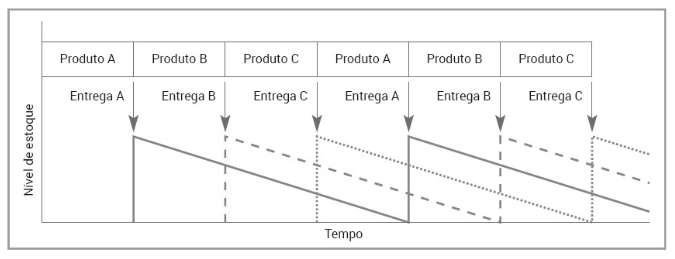
\includegraphics[width=0.8\textwidth]{imagens/Grafico_dente_de_serra.png}
    \caption{Gráfico dente de serra para múltiplos produtos (Fonte: Slack, Chambers e Johnston, 8ª ed.).}
    \label{fig:dente_serra}
\end{figure}

\subsection{Decisões de Volume e Timing com Apoio Externo}
As principais decisões operacionais envolvem definir quanto pedir (decisão de volume) e quando pedir (decisão de timing), buscando minimizar o esforço e os custos totais de reabastecimento. Para lidar com essa complexidade de forma eficiente, o restaurante adota uma estratégia de controle terceirizado, trabalhando em conjunto com uma empresa parceira externa especializada. Essa empresa processa as informações operacionais e emite relatórios analíticos regulares que indicam precisamente o que deve ou não ser adquirido em cada ciclo para a produção da parmegiana de carne, evitando o acúmulo desnecessário de farinha panko para empanamento ou a falta do queijo para o gratinamento, atuando na prática como o sistema de informação de estoque da operação para guiar as decisões de ressuprimento.

\subsection{Monitoramento, Feedback Financeiro e Regulação do Fluxo}
Por fim, o monitoramento contínuo é essencial para garantir o retorno financeiro e evitar perdas por deterioração, um risco crítico no setor de alimentos. A dinâmica com a empresa parceira fornece um mecanismo de intervenção direta: ela oferece feedback sobre o ganho real da operação e sobre a precificação dos fornecedores, indicando as opções mais competitivas do mercado para as compras dos ingredientes da parmegiana de carne. Além disso, regula o fluxo de entrada de insumos — sinalizando a interrupção de compras diante de acúmulos excessivos ou orientando adequação quando os níveis estão abaixo do necessário. Esse controle assegura estoques dimensionados de forma adequada, otimizando os custos globais de pedido e manutenção sem comprometer a capacidade do restaurante de entregar seus pratos.

% ============================================================
% 12. CAP 16 – MELHORAMENTO DA PRODUÇÃO
% ============================================================
\section{Cap. 16 – Melhoramento da Produção}

O capítulo trata do melhoramento da produção como uma responsabilidade central da gestão de operações, estruturada em elementos, abordagens, técnicas e gestão do processo de melhoria. 

\subsection{Melhoramento Incremental e Abordagem Colaborativa}
No restaurante, esse ciclo de melhoramento se manifesta de forma contínua e incremental — caracterizando uma filosofia próxima ao kaizen (Figura~\ref{fig:melhoramento_continuo}) —, especialmente no processo de desenvolvimento de novos pratos. A introdução de um item ao cardápio passa por uma reunião estruturada entre proprietários, gerentes, cozinheiros e o chef, onde a melhor ideia é selecionada coletivamente. A transição do papel para a prática é liderada pela própria cozinha, o que reforça o elemento de "inclusão de todos" e o desenvolvimento de relacionamentos internos entre as partes da operação ao testar a confecção e montagem de pratos como a parmegiana de carne.

\begin{figure}[htbp]
    \centering
    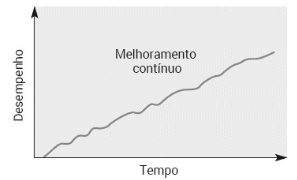
\includegraphics[width=0.7\textwidth]{imagens/Melhoramento_Contínuo.png}
    \caption{Relação entre melhoramento contínuo (kaizen) e o tempo (Fonte: Slack, Chambers e Johnston, 8ª ed.).}
    \label{fig:melhoramento_continuo}
\end{figure}

\subsection{Coleta de Evidências, Feedbacks e Ciclo PDCA}
A coleta e o uso de evidências também compõem o esforço de melhoramento do restaurante, alinhando-se ao elemento de solução de problemas baseada em evidência. O feedback dos clientes é obtido por dois canais — Google e tablets no próprio estabelecimento —, funcionando como instrumentos de monitoramento contínuo que permitem detectar desvios de qualidade especificamente na parmegiana de carne (como textura do empanamento) e orientar intervenções rápidas no processo. Esse mecanismo aproxima a operação de um ciclo PDCA informal, no qual os resultados percebidos pelos clientes retroalimentam as decisões operacionais da equipe, conforme ilustrado no ciclo clássico de melhoramento (Figura~\ref{fig:pdca}).

\begin{figure}[htbp]
    \centering
    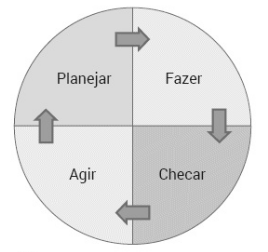
\includegraphics[width=0.45\textwidth]{imagens/Ciclo_PDCA.png}
    \caption{O Ciclo PDCA de melhoramento de processos (Fonte: Slack, Chambers e Johnston, 8ª ed.).}
    \label{fig:pdca}
\end{figure}

\subsection{Vinculação à Estratégia e Padronização de Etapas}
Por fim, a gestão do melhoramento exige organização e vinculação à estratégia da operação. A adoção da gramatura pré-porcionada para as proteínas da parmegiana de carne exemplifica um melhoramento incremental que reduziu o tempo de confecção do prato principal para aproximadamente 10 minutos, impactando diretamente a experiência do cliente. Esse tipo de melhoria localizada, simples e de baixo custo, ilustra como técnicas analíticas relativamente simples — como a padronização de etapas do processo (separação, empanamento com ovo e farinha panko, fritura, adição de molho e queijo, e gratinamento) — podem gerar ganhos expressivos de desempenho sem a necessidade de mudanças radicais ou de ruptura.


% ============================================================
% 13. PROPOSTA DE MELHORIA (DO GRUPO)
% ============================================================
\section{Proposta de Melhoria}

A principal proposta de melhoria para o Restaurante e Bar Tarumã foca na mitigação do seu maior desafio operacional relatado: a falta de padronização no preparo e na montagem da parmegiana. Segundo a teoria de Gestão da Qualidade e de Operações, abordada por Slack \textit{et al.} (2009) e Krajewski \textit{et al.} (2012), a qualidade de conformidade significa entregar o produto consistente com suas especificações de projeto, minimizando a variabilidade para garantir que todo cliente receba exatamente a mesma experiência. A dificuldade de padronização indica que a operação possui alta dependência do conhecimento tácito dos funcionários e pouca formalização de seus métodos.

Para solucionar essa questão, propõe-se a implementação de Procedimentos Operacionais Padrão (POPs) integrados a ferramentas de Gestão Visual diretamente nas estações de trabalho da cozinha. Na prática, isso se traduz na elaboração de Fichas Técnicas Operacionais afixadas no setor de montagem e cocção. Essas fichas não devem ser apenas textuais, mas sim painéis visuais que contenham fotos do prato ideal (padrão de saída), os tempos exatos estipulados para fritura e gratinação na salamandra, e as gramaturas rigorosas de cada componente.

Adicionalmente, como apoio a essa padronização, sugere-se a introdução de técnicas de controle baseadas no princípio de Poka-Yoke (sistemas à prova de erros). Isso pode ser feito através da padronização dos utensílios de medição: adotar conchas específicas que comportem o volume exato de molho de tomate por prato e recipientes pré-medidos para a quantidade de queijo e batatas fritas. Ao transferir o controle de qualidade da "intuição" do cozinheiro para o sistema físico e visual, o restaurante reduzirá a variabilidade da produção. Essa ação melhorará o objetivo de desempenho de qualidade (sabor e apresentação consistentes) e protegerá o objetivo de custos, evitando o desperdício ou a variação na margem de lucro causada pelo superporcionamento involuntário.


% ============================================================
% 14. CONSIDERAÇÕES FINAIS
% ============================================================
\section{Considerações Finais}

A realização desta visita técnica e a consequente elaboração deste relatório proporcionaram uma oportunidade valiosa de conectar os modelos teóricos de Gestão da Produção e Qualidade à dinâmica real e acelerada de um serviço de alimentação. Um dos pontos mais interessantes da jornada do grupo foi observar como conceitos acadêmicos complexos de estratégia operacional e gestão de capacidade se materializam em decisões pragmáticas do dia a dia, como a definição de um cardápio enxuto, o pré-porcionamento milimétrico de bifes e a escolha de terceirizar a inteligência de suprimentos.


% ============================================================
% REFERÊNCIAS
% ============================================================
\newpage
\section*{Referências}
\addcontentsline{toc}{section}{Referências}

\begin{description}[leftmargin=0pt, labelwidth=0pt, itemsep=6pt]

  \item SLACK, Nigel; CHAMBERS, Stuart; JOHNSTON, Robert.
    \textit{Administração de produção.} 8.~ed. São Paulo: Atlas.

  \item KRAJEWSKI, Lee~J.; RITZMAN, Larry~P.; MALHOTRA, Manoj~K.
    \textit{Administração de produção e operações.} 8.~ed.
    São Paulo: Pearson, 2012. 615~p.
    ISBN~9788576051725.

  \item SLACK, Nigel; CHAMBERS, Stuart; JOHNSTON, Robert.
    \textit{Administração de produção.} 3.~ed.
    São Paulo: Atlas, 2009. 703~p.
    ISBN~9788522453535.

  \item GIRI, Sunita.
    \textit{Operations Research and Quality Management.}
    ABD Publishers, 2010.
    Disponível em: \url{http://site.ebrary.com/lib/univbrasilia/docDetail.action?docID=10416308}.

\end{description}

\subsection*{Bibliografia Complementar}

\begin{description}[leftmargin=0pt, labelwidth=0pt, itemsep=6pt]

  \item ANTUNES, Junico.
    \textit{Sistemas de produção: conceitos e práticas para projeto e gestão da produção enxuta.}
    Porto Alegre: Bookman, 2008. 326~p.
    ISBN~9788577801169.

  \item BALLESTERO-ALVAREZ, María Esmeralda.
    \textit{Gestão de qualidade: produção e operações.}
    2.~ed. São Paulo: Atlas, 2012. 460~p.
    ISBN~9788522471058.

  \item BATALHA, Mário Otávio (Org.).
    \textit{Introdução à engenharia de produção.}
    Rio de Janeiro: Elsevier, 2008. 312~p.
    ISBN~9788535223304.

  \item DE~SORDI, José Osvaldo.
    \textit{Gestão por processos: uma abordagem da moderna administração.}
    3.~ed. São Paulo: Saraiva, 2012. 338~p.
    ISBN~9788502175518.

  \item FERREIRA, Ayrton Sérgio Rochedo.
    \textit{Modelagem organizacional por processos.}
    Rio de Janeiro: Mauad X, 2010. 270~p.
    ISBN~9788574783239.

\end{description}

\end{document}
